% Chapter 2

\chapter{Navigation Among Movable Obstacles: state of the art} % Main chapter title

\label{Chapter2} % For referencing the chapter elsewhere, use \ref{Chapter2}

\section{Determining appropriate comparison criteria}

\begin{figure}[H]
\centering
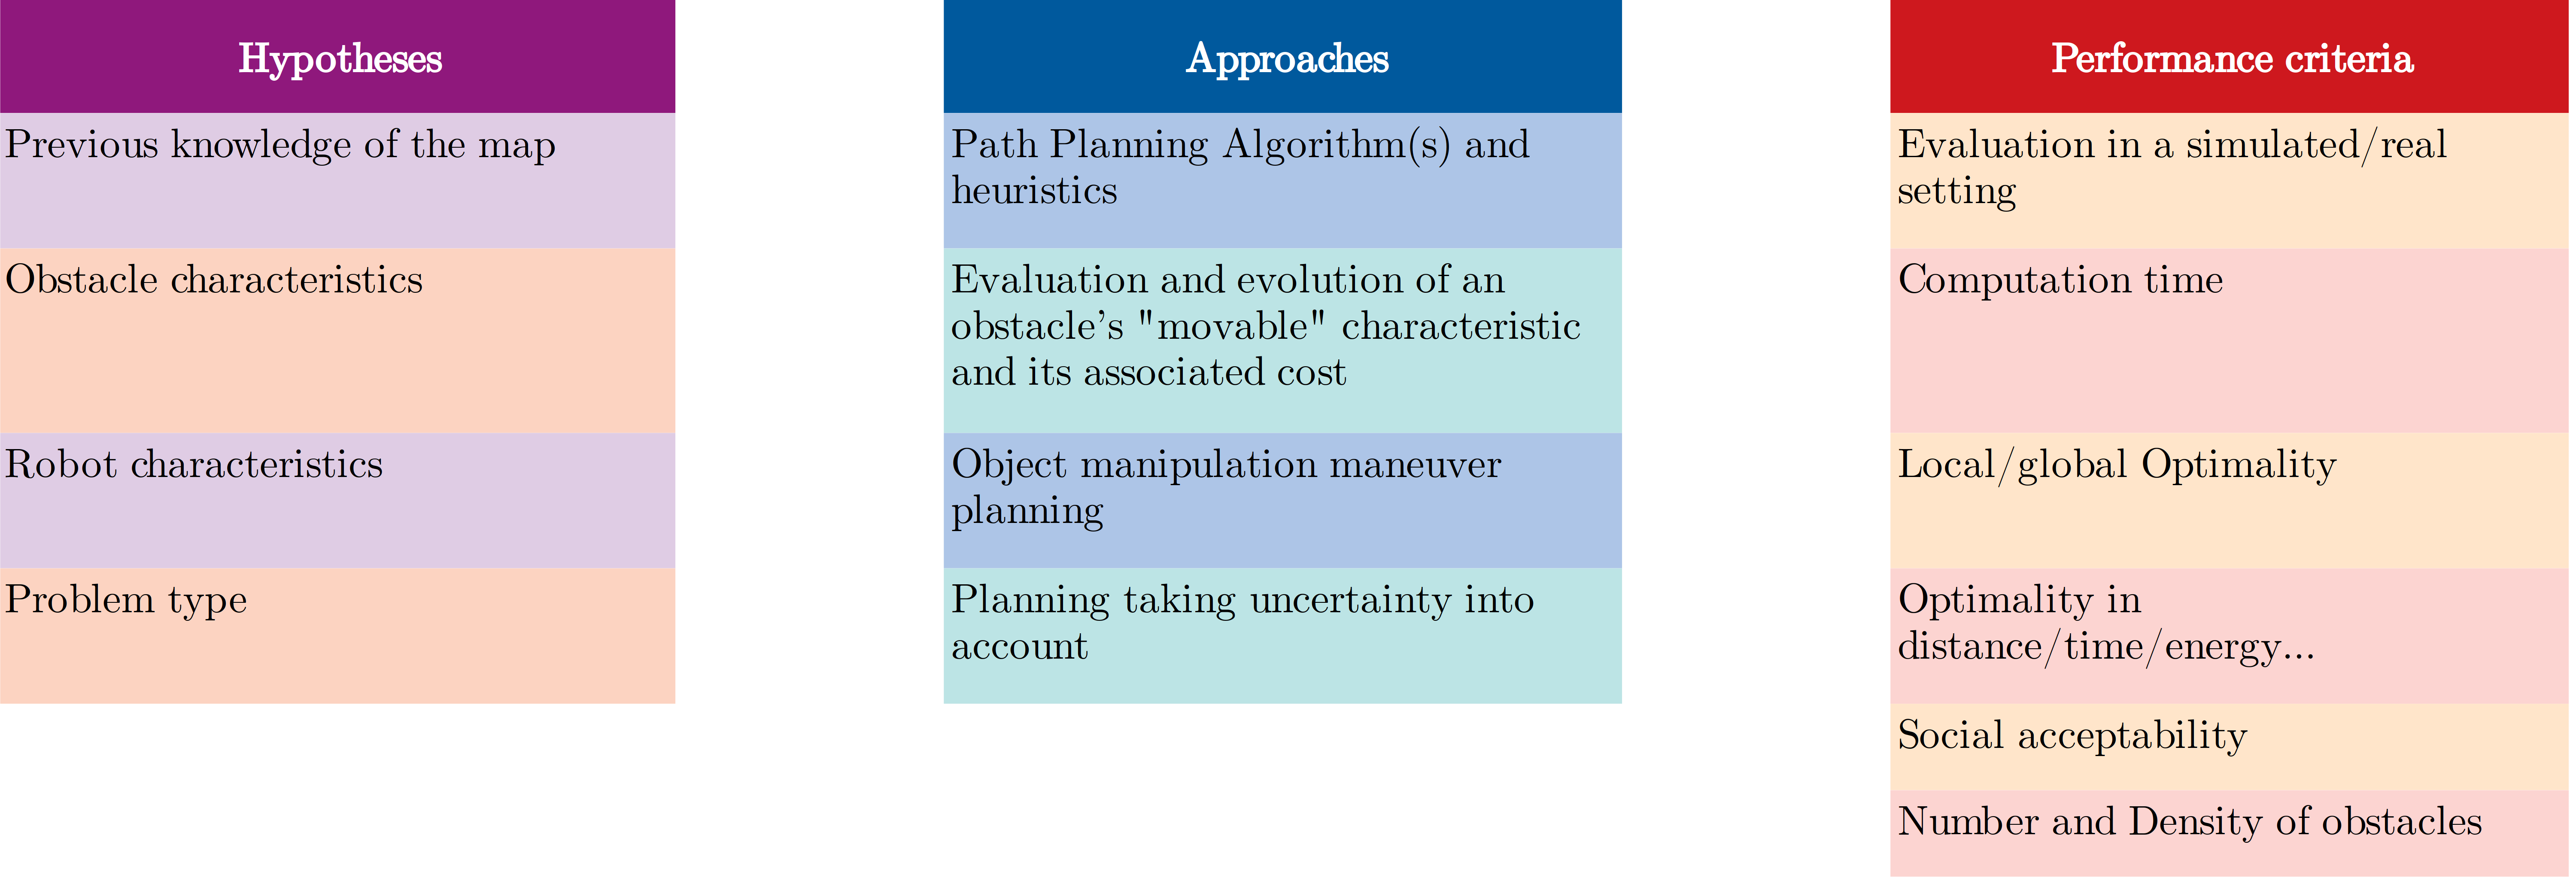
\includegraphics[width=15cm]{Comparison_Table/comparison_criteria}
\decoRule
\caption[Comparison criteria listing]{Comparison criteria, sorted by type: hypotheses, approaches and performance criterias}
\label{fig:comparison_criteria}
\end{figure}

\subsection{Hypotheses}

%% Here explain in more detail why these comparison criteria

\subsection{Approaches}

%% Here explain in more detail why these comparison criteria

\subsection{Performance criteria}

%% Here explain in more detail why these comparison criteria

\section{Comparison and cross-comparison}

\subsection{Comparison tables}

%% Here explain acronyms and abbreviations

%% Here insert the basic comparison tables

%% Here insert mention of and link to the cross comparison tables in the appendices

%% Here insert mention of and link to the detailed comparison table available in the appendices

\subsection{Conclusions}



\subsection{Situating our work in the established context}
